\section{Matter effects and crust density}
\label{app:crust_density}

To check the effect of the error on the average crust density \cite{MatterEffect} a number of fits of \deltacp were performed varying this value. \Crefrange{fig:matter_nh}{fig:matter_ih} show the effect of varying the average crust density between 2.5, 2.6 and $2.7\text{ g cm}^{-3}$ in normal and inverted hierarchy respectively. \num{1e4} marginalisation toys were generated with the average crust density fixed at the value of $2.6\text{ g cm}^{-3}$, whilst fits were performed using the Asimov A data set where the crust density was varied using the aforementioned values. The effect on the fit of \deltacp can be seen to be small, supporting the use of a fixed value for the average crust density.

\begin{figure*}[htb]
	\center
	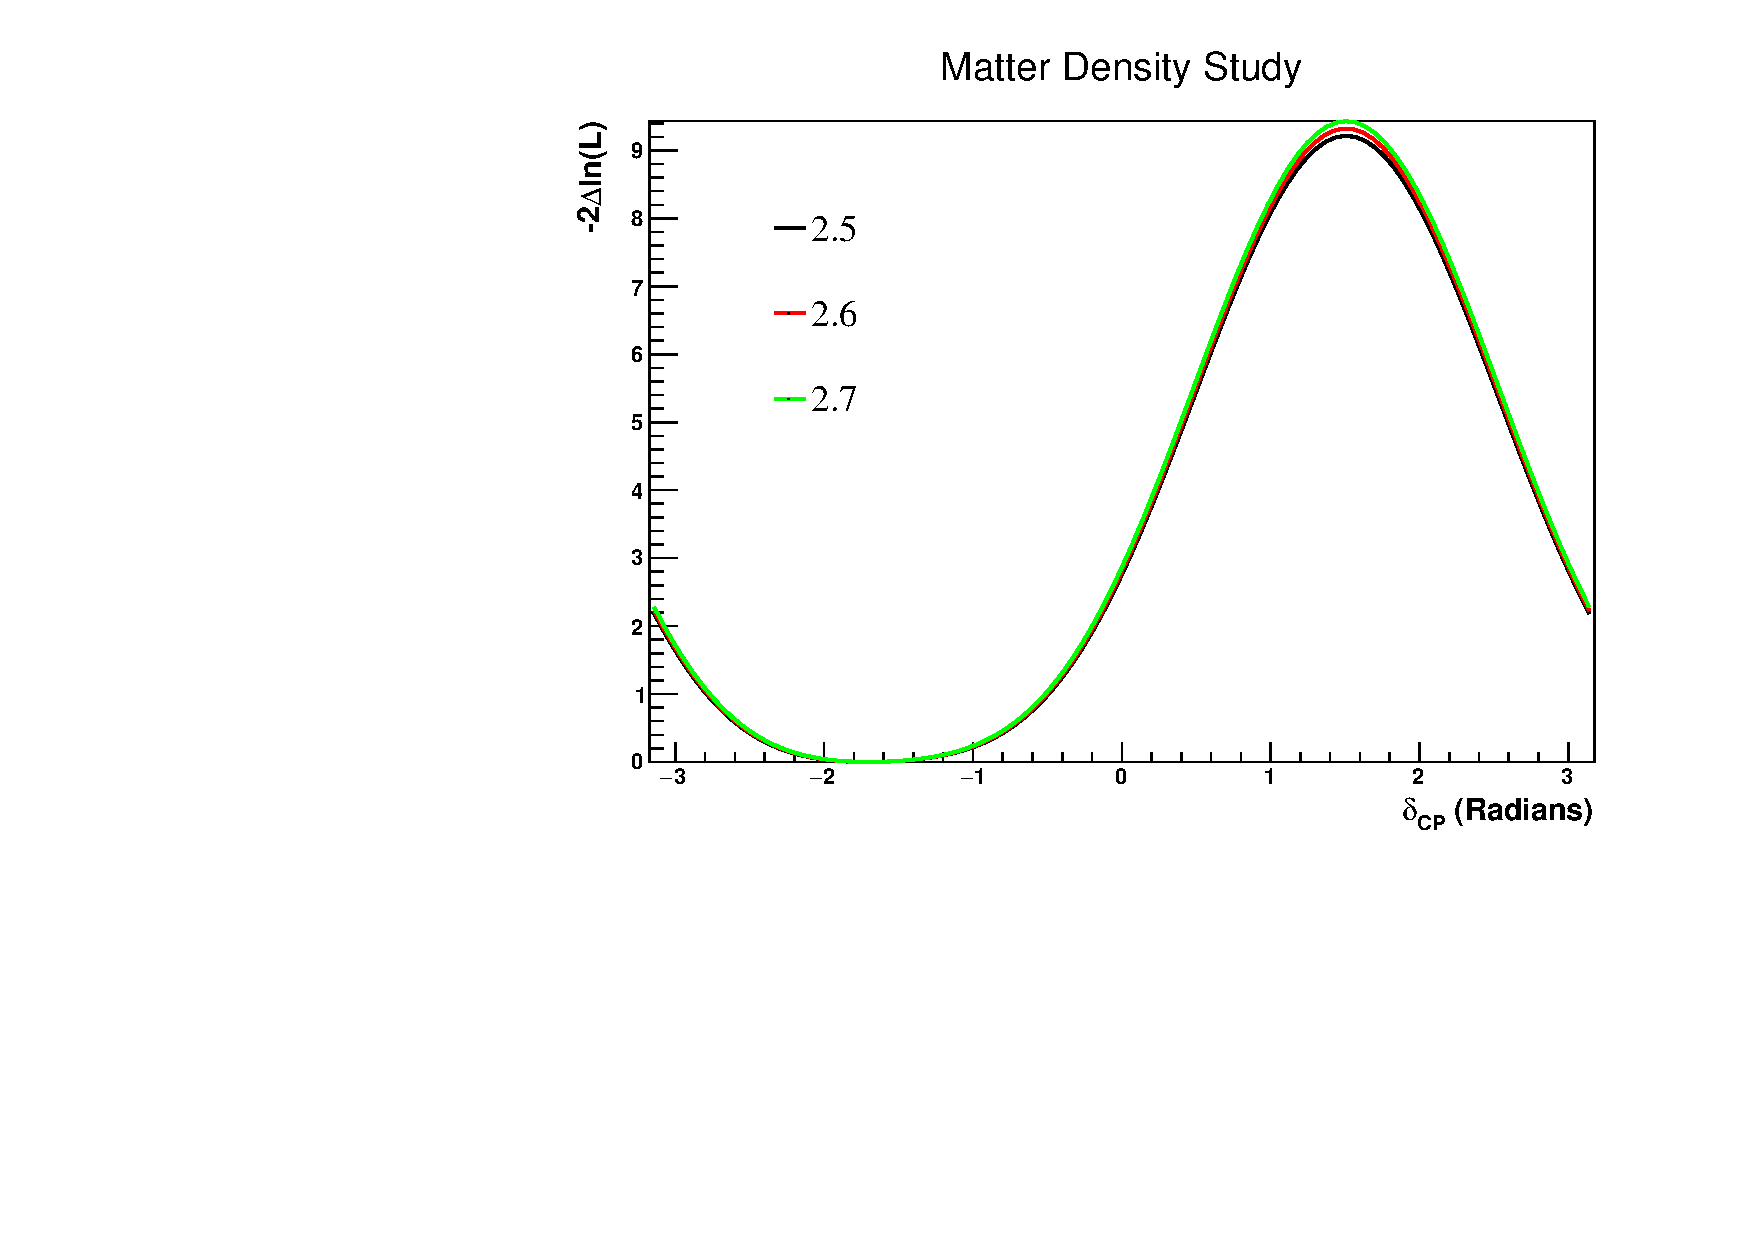
\includegraphics[width=0.7\textwidth]{studies/matter/matter_normal}
	\caption{Fits of \deltacp using the Asimov A data set whilst varying the average crust density in normal hierarchy for 10K marginalisation toys.}
	\label{fig:matter_nh}
\end{figure*}

\begin{figure*}[htb]
	\center
	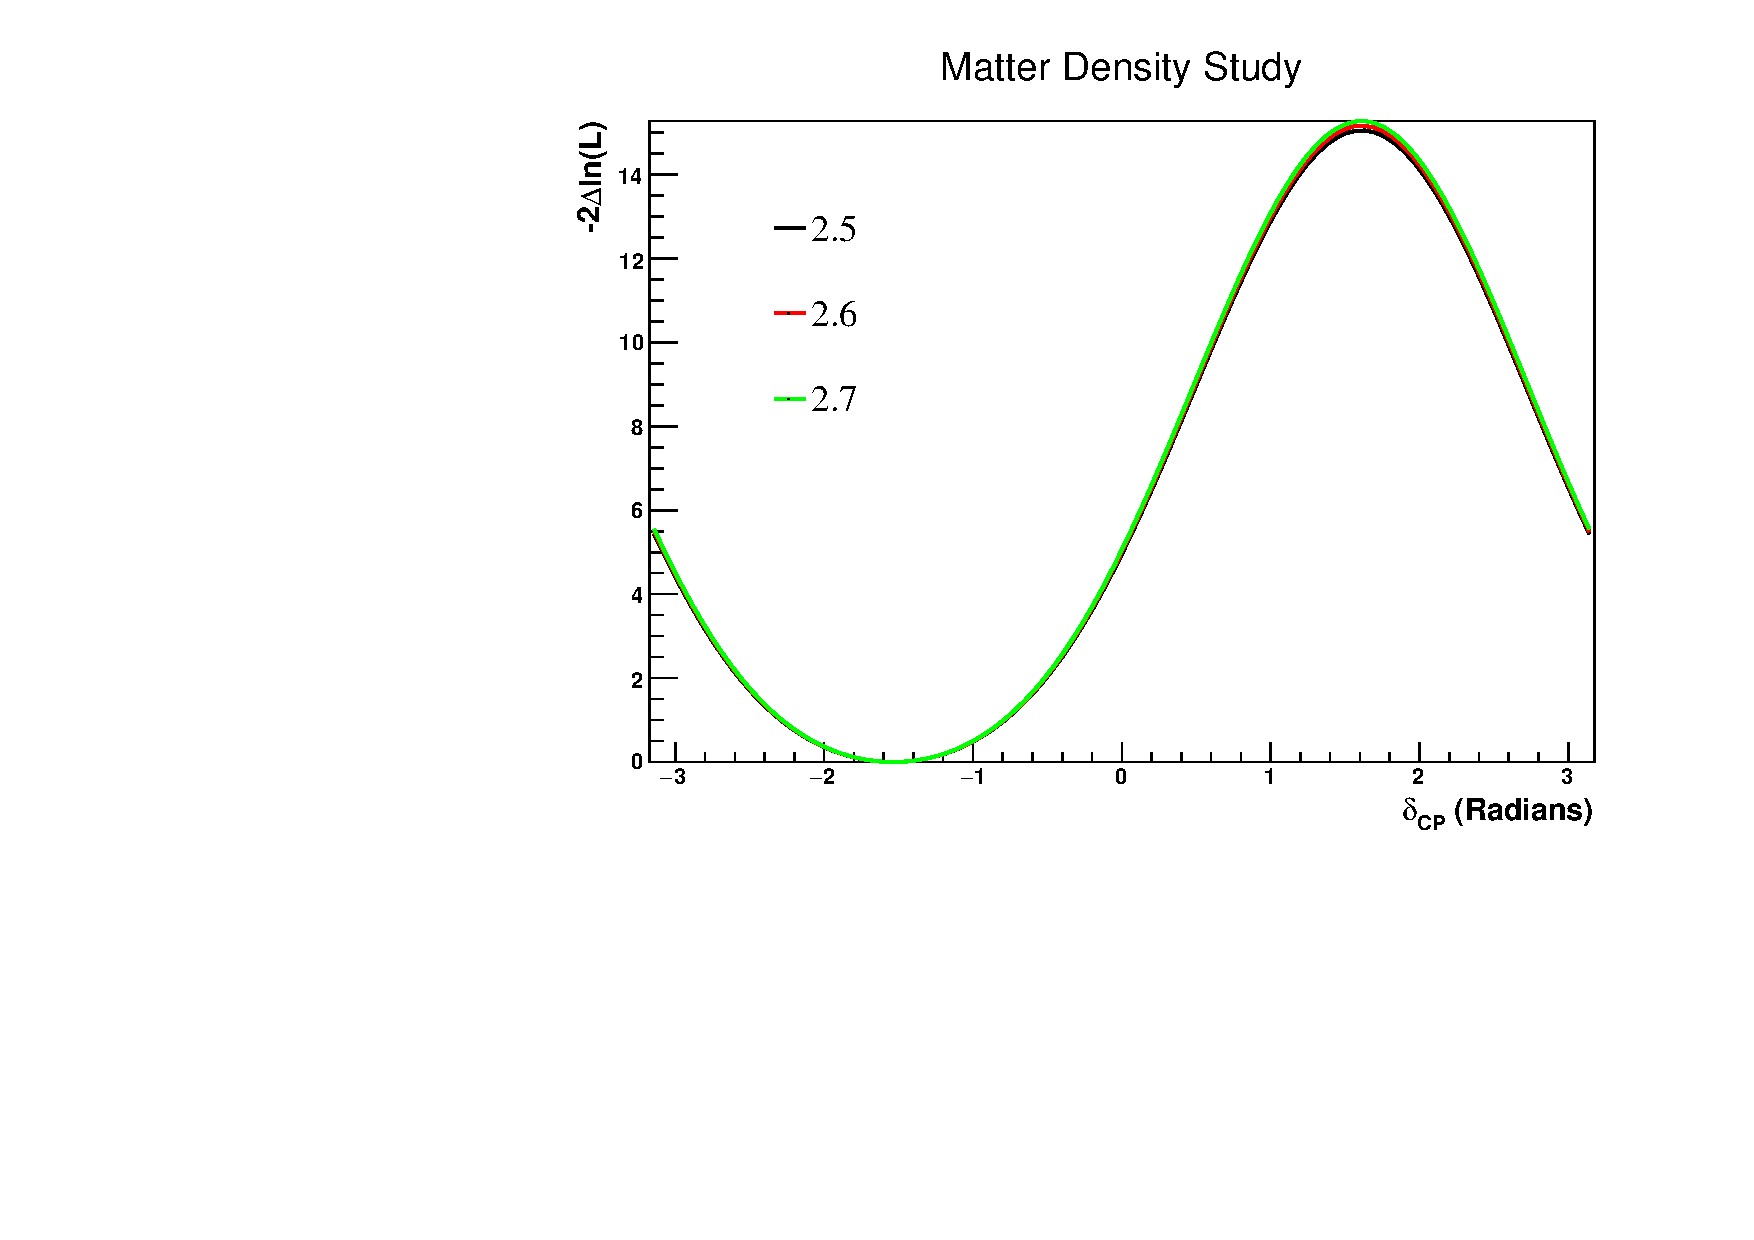
\includegraphics[width=0.7\textwidth]{studies/matter/matter_inverted}
	\caption{Fits of \deltacp using the Asimov A data set whilst varying the average crust density in inverted hierarchy for 10K marginalisation toys.}
	\label{fig:matter_ih}
\end{figure*}
\clearpage